\chapter{Instrukcja użytkownika}
\section{Początki pracy  z narzędziem}
Zanim zacznie się pracować z narzędziem, należy zainstalować
wszystkie wykorzystywane przez nie zależności. Instalacja została 
usprawniona wykorzystując Vagrant oraz Ansible, ale można ją przeprowadzić
również bez tych technologii. Oba te sposoby oraz późniejsza praca z narzędziem,
która zależy od wybranego sposobu instalacji są opisane poniżej.

\subsection{Projekt na Google Cloud}
Aplikacja używa Google Forms API do zarządzania formularzami na dysku Google
użytkownika i z tego powodu potrzebuje danych uwierzytelniających do 
komunikacji z tym API. Można je uzyskać zakładając projekt na Google Cloud.
Dokładne instrukcje można znaleźć w poradnikach w dokumentacji Google, 
a w tej pracy spróbuję krótko opisać ten proces: 

\begin{itemize}
  \item załóż nowy projekt
    \begin{itemize}
      \item zaloguj się do konsoli Google Cloud,
      \item znajdź przycisk ,,Wybierz Projekt'',
      \item w nowym oknie naciśnij przycisk ,,Nowy Projekt'',
      \item wpisz nazwę projektu oraz lokalizację, a następnie naciśnij ,,Utwórz'',
    \end{itemize}
  \item  Dodaj Google Forms API do projektu
    \begin{itemize}
      \item w menu po lewej stronie wybierz ,,Wyświetl Wszystkie Usługi'',
      \item w sekcji ,,Zarządzanie'' wybierz ,,Interfejsy API i usługi'',
      \item wybierz swój projekt,
      \item kliknij ,,Interfejsy API i usługi'',
      \item wyszukaj ,,Google Forms API'',
      \item w szczegółach Google Forms API kliknij ,,Włącz'',
    \end{itemize}
  \item wygenereuj Klucz interfejsu API
    \begin{itemize}
      \item przejdź do strony projektu,
      \item w menu po lewej stronie wybierz ,,Dane logowania'',
      \item kliknij ,,Create Credentials'', a potem ,,Klucz interfejsu API'',
      \item zapisz klucz w pliku i zachowaj na później,
    \end{itemize}
  \item skonfiguruj ekran zgody
    \begin{itemize}
      \item przejdź do strony projektu,
      \item ponownie kliknij ,,Create Credentials'', a potem 
            ,,Identyfikator Klienta OAuth'',
      \item kliknij ,,Skonfiguruj Ekran Zgody'',
      \item jako typ użytkownika wybierz ,,Zewnętrzny'' i kliknij ,,Utwórz'',
      \item wpisz nazwę aplikacji, adresy e-mail i kliknij ,,Zapisz i kontynuuj'',
      \item kliknij ,,Dodaj lub usuń zakres'',
      \item w ,,Filtruj'' wpisz ,,Google Forms API'',
      \item zaznacz zakresy ,,forms.body'' i ,,forms.responses.readonly'',
      \item kliknij ,,Zaktualizuj'', następnie ,,Zapisz i kontynuuj'',
      \item dodaj swój adres konta Google do użytkowników testowych, kliknij
      ,,Zapisz i kontynuuj'' i na końcu ,,Powrót do panelu'',
    \end{itemize}
  \item wygeneruj identyfikator klienta OAuth
    \begin{itemize}
      \item przejdź do strony projektu,
      \item wybierz ponownie ,,Dane Logowania'', ,,Create Credentials''
            i ,,Identyfikator Klienta OAuth'',
      \item jako typ aplikacji wybierz ,,Aplikacja internetowa'', dodaj URI 
            \\ \texttt{http://localhost:3000/oauth2callback} do sekcji ,,Autoryzowane 
            identyfikatory URI przekierowania'' i kliknij ,,Utwórz'',
      \item wybierz ,,Pobierz JSON''.
    \end{itemize}
\end{itemize}

\subsection{Imgur API}
Aplikacja używa Imgur API, żeby wygenerować linki zewnętrzne obrazków
z formułami matematycznymi, z których pobiera je serwer Google. Do komunikacji
z Imgur API również potrzebujemy danych uwierzytelniania:
\begin{itemize}
  \item zaloguj się do Imgur,
  \item odwiedź stronę \href{https://api.imgur.com/}{Imgur API},
  \item znajdź ,,Register an application'',
  \item wypełnij dane, jako typ autoryzacji wybierz ,,OAuth2 authorization without
  a callback URL'',
  \item skopiuj Client ID i Client secret i zachowaj na później.
\end{itemize}

\subsection{Repozytorium}
Teraz należy sklonować \href{https://github.com/arozkrut/forms-apps}
{repozytorium projektu} --- github.com/arozkrut/forms-app.
Następnie w pobranym repozytorium w katalogu \texttt{forms-app/src/credentials}
stwórz pliki:
\begin{itemize}
  \item \texttt{api\_key.txt}: wklej tu klucz interfejsu API, tak żeby plik był
  postaci
  \begin{verbatim}
    key=<uzyskany klucz>
  \end{verbatim}
  Klucz służy do identyfikacji aplikacji podczas wysyłania zapytań do Google Forms API. 
  Proces generacji klucza interfejsu API został opisany wczesniej w tym rozdziale.
  \item \texttt{credentials.json}: wklej tu zawartość pobranego pliku JSON.
  Plik zawiera dane uwierzytelniające, które również są używane przy wysyłaniu
  zapytań do Google Forms API. 
  Proces generacji pliku JSON został opisany wcześniej w tym rozdziale.
  \item \texttt{imgur\_credentials.txt}: wklej tu Client ID i Client secret,
  tak żeby plik był postaci:
  \begin{verbatim}
    ClientID: <Client ID>
    ClientSecret: <Client secret>
  \end{verbatim}
  Identyfikator oraz sekret służą do identyfikacji aplikacji podczas wysyłania zapytań
  do Imgur API. Proces generacji identyfikatora oraz sekretu został opisany wcześniej
  w tym rozdziale.
\end{itemize}

\subsection{Instalacja z Vagrant}
Jeśli masz już zainstalowany Vagrant wystarczy, że w głównym katalogu projektu
(tym z \texttt{Vagrantfile}) użyjesz polecenia \texttt{vagrant up}. Skrypt
Ansible zainstaluje wszystkie potrzebne zależności i uruchomi wszystkie
aplikacje. Ważne jest, że projekt potrzebuje portów 3000, 9090 i 9091.
Jeśli któryś z nich jest już zajęty narzędzie nie uruchomi się. Porty 9090 i 9091
można zmienić na inne, ale portu 3000 niestety nie. Opis jak to zrobić można znaleźć
w sekcji ,,Porty''. Instalacja może
chwilę potrwać. Po jej zakończeniu wyświetli się wiadomość z linkiem prowadzącym
do strony uwierzytelniania Google, gdzie trzeba wybrać konto Google, na którym
będą przechowywane formularze oraz wyrazić zgodę na nadanie aplikacji dostępu do
formularzy na tym koncie. Następnie w przeglądarce należy odwiedzić adres
\href{http://localhost:9091}{http://localhost:9091}, gdzie działa interfejs
użytkownika. Narzędzie jest gotowe do pracy.

\subsection{Instalacja bez Vagrant}
Jeśli użytkownik chce korzystać z narzędzia bez zainstalowanego Vagrant, musi on
sam zainstalować wszystkie zależności: Python 3, \LaTeX{}, poppler-utils, biblioteki
do języka Python opisane w poprzednim rozdziale, nodejs, npm. Następnie w katalogach
\texttt{forms-app} oraz \texttt{forms-app-ui} należy wydać polecenie \texttt{npm i}.
Teraz należy włączyć serwer NodeJS poleceniem \texttt{node src/server.js} 
(koniecznie w katalogu \texttt{forms-app}). Serwer korzysta z portów 9090 i 3000, 
więc przed uruchomieniem należy upewnić się, że są one niezajęte. Port 9090 można
zmienić na inny, ale 3000 już nie. Opis jak to zrobić można znaleźć w sekcji ,,Porty''.
Po uruchomieniu serwera w przeglądarce powinna otworzyć się
strona uwierzytelniania Google, gdzie trzeba wybrać konto Google, na którym
będą przechowywane formularze oraz wyrazić zgodę na nadanie aplikacji dostępu do
formularzy na tym koncie. Po tym w katalogu \texttt{src/forms-app-ui}
należy włączyć serwer interfejsu użytkownika poleceniem \texttt{npm start}, który
uruchomi się pod adresem \href{http://localhost:9091}{http://localhost:9091}.
Port 9091 na którym działa aplikacja można również zmienić na inny.
Po odwiedzeniu \href{http://localhost:9091}{http://localhost:9091} w przeglądarce
można zacząć pracować z narzędziem.

\section{Porty}
Narzędzie korzysta z trzech portów: 9090, 9091 oraz 3000. Dwa pierwsze można
zmienić edytując kilka linijek w kodzie, ale portu 3000 niestety nie da się zmienić
na inny. Jest on wykorzystywany przez bibliotekę, służącą do autoryzacji aplikacji
i użytkownika w serwerach Google i ta biblioteka nie udostępnia sposobu 
na zmianę tego portu. Niezależnie, czy narzędzie jest instalowane używając Vagranta,
czy nie pierwsze kroki, żeby zmienić porty 9090 i 9091 są takie same:
\begin{itemize}
  \item zmiana portu 9090: 
    \begin{itemize}
      \item w pliku \texttt{forms-app/src/server.js} znajdź zmienną
        \texttt{port} i zmień jej wartość,
      \item w plikach
        \begin{itemize}
          \item \texttt{forms-app-ui/src/App.tsx}
          \item \texttt{forms-app-ui/src/components/FormCard.tsx}
        \end{itemize}
        znajdź zmienną \texttt{SERVER\_BASE\_URL} i zmień port na inny,
    \end{itemize}
  \item zmiana portu 9091:
    \begin{itemize}
      \item w pliku \texttt{forms-app-ui/package.json} w \texttt{scripts}, 
            \texttt{start} zmień \texttt{PORT=9091} na inny port.
    \end{itemize}
\end{itemize}

Jeśli narzędzie jest instalowane z użyciem Vagranta w pliku \texttt{Vagrantfile}
należy dodać nowe porty. Pod linijkami:
\begin{verbatim}
  config.vm.network :forwarded_port, guest: 80, host: 8001
  config.vm.network :forwarded_port, guest: 9090, host: 9090
  config.vm.network :forwarded_port, guest: 3000, host: 3000
  config.vm.network :forwarded_port, guest: 9091, host: 9091
\end{verbatim}
dla każdego nowego portu należy dodać linijkę:
\begin{verbatim}
  config.vm.network :forwarded_port, guest: <NOWY_PORT>, host: <NOWY_PORT>
\end{verbatim}
Po wykonaniu tych kroków należy zresetować obie aplikacje lub maszynę wirtualną
poleceniem \texttt{vagrant reload}.

\section{Praca z narzędziem}

\subsection{Schemat pliku kodującego (JSON)}
Poniżej znajduje się rozpisany schemat kodowania: 
\begin{figure}[H]
\begin{lstlisting}[language=json,firstnumber=1]
{
  "title": "string",
  "description": "string",
  "startDate": "string",
  "endDate": "string",
  "shuffleAnswers": "boolean",
  "questions": [{
    "type": "string", 
    "text": "string",
    "tex" : "boolean",
    "answers": [{
      "text" : "string",
      "tex" : "boolean",
      "correct" : "boolean"
    }],
    "points": "number"
    "pointsArray": "array"
  }]
}
\end{lstlisting}
\end{figure}
Jest to opis tych wartości, które mogą być użyte --- nie wszystkie są jednak 
wymagane. Poniżej znajduje się szczegółowy opis pól i wartości:
\begin{itemize}
  \item{title} -- wartość tekstowa, odpowiada nagłówkowi formularza --- 
  \textbf{pole wymagane},
  \item{description} -- wartość tekstowa, krótki opis formularza, który
  pojawi się pod tytułem ---  \textbf{pole opcjonalne},
  \item{startDate} -- wartość tekstowa, data planowanego rozpoczęcia testu
  w formacie ISO. To pole służy tylko do odrzucania odpowiedzi, które zostały
  przesłane przed podaną datą podczas oceniania ---  \textbf{pole opcjonalne},
  \item{endDate} -- wartość tekstowa, data planowanego zakończenia testu
  w formacie ISO. To pole służy tylko do odrzucania odpowiedzi, które zostały
  przesłane po podanej dacie podczas oceniania ---  \textbf{pole opcjonalne},
  \item{shuffleAnswers} -- wartość boolowska, informacja o tym, czy odpowiedzi
  dla każdego pytania powinny zostać przetasowane dla każdego wyświetlenia
  formularza. Niestety na ten moment Google Forms API nie udostępnia opcji
  tasowania pytań, można ją jedynie włączyć ręcznie w ustawieniach formularza
  na stronie Google: settings -> presentation -> Shuffle question order
  ---  \textbf{pole opcjonalne},
  \item{questions} -- tablica, której każde pole zawiera informacje dotyczące
  jednego pytania --- \textbf{pole wymagane}. \\Poniżej znajdują się wartości
  kodujące pojedyncze pytanie:
  \begin{itemize}
    \item{type} -- pole tekstowe dotyczące typu kodowanego pytania.
    Dopuszczalne wartości:
    \begin{itemize}
      \item ,,checkBox'' -- pytanie zamknięte wielokrotnego wyboru,
      \item ,,grid'' -- pytanie typu ,,prawda/fałsz'',
      \item ,,list'' -- zamknięte jednokrotnego wyboru,
      \item ,,text'' -- otwarte.
    \end{itemize}
    \textbf{pole wymagane},
    \item{text} -- zawiera treść pytania w formie tekstowej. Może zawierać wstawki
    z \LaTeX{}'a. Należy jednak pamiętać, że JavaScript traktuje symbol ,,$\backslash$''
    jako specjalny --- wszystkie wystąpienia ,,$\backslash$'' należy więc zastąpić
    ,,$\backslash\backslash$'' --- \textbf{pole wymagane},
    \item{tex} -- wartość boolowska, jeśli \textbf{true} treść pytania (text) będzie
    konwertowana do obrazu z zachowaniem konwersji symboli matematycznych i innych
    wstawek z \LaTeX{}'a z biblioteki standardowej --- \textbf{pole wymagane},
    \item{answers} -- tablica, każde pole zawiera jedną z możliwych odpowiedzi w
    następującej formie:
    \begin{itemize}
      \item text -- pole tekstowe, treść danej odpowiedzi; podobnie jak w treści
        pytania wszystkie wystąpienia ,,$\backslash$'' należy zastąpić 
        ,,$\backslash\backslash$'',
      \item tex -- wartość boolowska, jeśli \textbf{true} treść odpowiedzi (text) będzie
      konwertowana do obrazu z zachowaniem konwersji symboli matematycznych i innych
      wstawek z \LaTeX{}'a z biblioteki standardowej, tylko dla pytań typu list i checkBox,
      \item correct -- wartość boolowska wskazująca czy dana odpowiedź jest prawidłowa.
      Domyślna wartość: false.
    \end{itemize} 
    --- \textbf{pole opcjonalne},
    \item{points} -- wartość numeryczna, odpowiada liczbie punktów przyznawanej za
    poprawą odpowiedź na pytanie (tylko dla pytań typu list)
    --- \textbf{pole opcjonalne},
    \item{pointsArray} -- tablica z wartościami numerycznymi, odpowiada liczbie punktów
    przyznawanej za poprawne odpowiedzi na pytanie (tylko dla pytań typu checkBox i grid),
    przykładowo wartość $ [0, 1, 3] $ wskazuje, że jeśli nie zostanie wybrana żadna dobra
    odpowiedź, zostanie przyznane 0 punktów, jeśli zostanie udzielona jedna dobra odpowiedź,
    zostanie przydzielony 1 punkt i jeśli zostaną udzielone dwie dobre odpowiedzi, zostaną
    przydzielone 3 punkty
    --- \textbf{pole opcjonalne}.
  \end{itemize}
\end{itemize}

\subsection{Automatyczne ocenianie}
Pytania typu list, checkBox i grid mogą zostać automatycznie ocenione i wyniki mogą zostać
pobrane w formacie JSON lub pliku Excel. Jeśli chcemy, żeby odpowiedzi zostały ocenione
musimy ręcznie ustawić zbieranie adresów email w ustawieniach formularza. Google Forms API
niestety na ten moment nie udostępnia możliwości zrobienia tego automatycznie. Sposób
oceniania zależy od typu pytania:
\begin{itemize}
  \item \textbf{list}: jeśli zostanie zaznaczona poprawna odpowiedź, odpowiadający uzyska
  całość punktów z pola \texttt{points}, w przeciwnym przypadku otrzyma 0 punktów,
  \item \textbf{checkBox}: zliczane są poprawnie zaznaczone odpowiedzi i od tej liczby
  odejmuje się liczbę niepoprawnie zaznaczonych odpowiedzi. Jeśli uzyskana liczba jest
  mniejsza od zera, podstawiamy za nią 0. Następnie z tablicy
  \texttt{pointsArray} z indeksu równego poprzednio uzyskanej liczbie odczytuje się liczbę
  uzyskanych punktów,
  \item \textbf{grid}: zliczane są poprawnie udzielone odpowiedzi i z indeksu równego
  tej liczbie odczytuje się liczbę uzyskanych punktów w tablicy \textbf{pointsArray}.
\end{itemize} 

\subsection{Obsługa narzędzia}
Po uruchomieniu użytkownik widzi stronę w przeglądarce, jak na zdjęciu poniżej:
\begin{figure}[H]
 \centering
  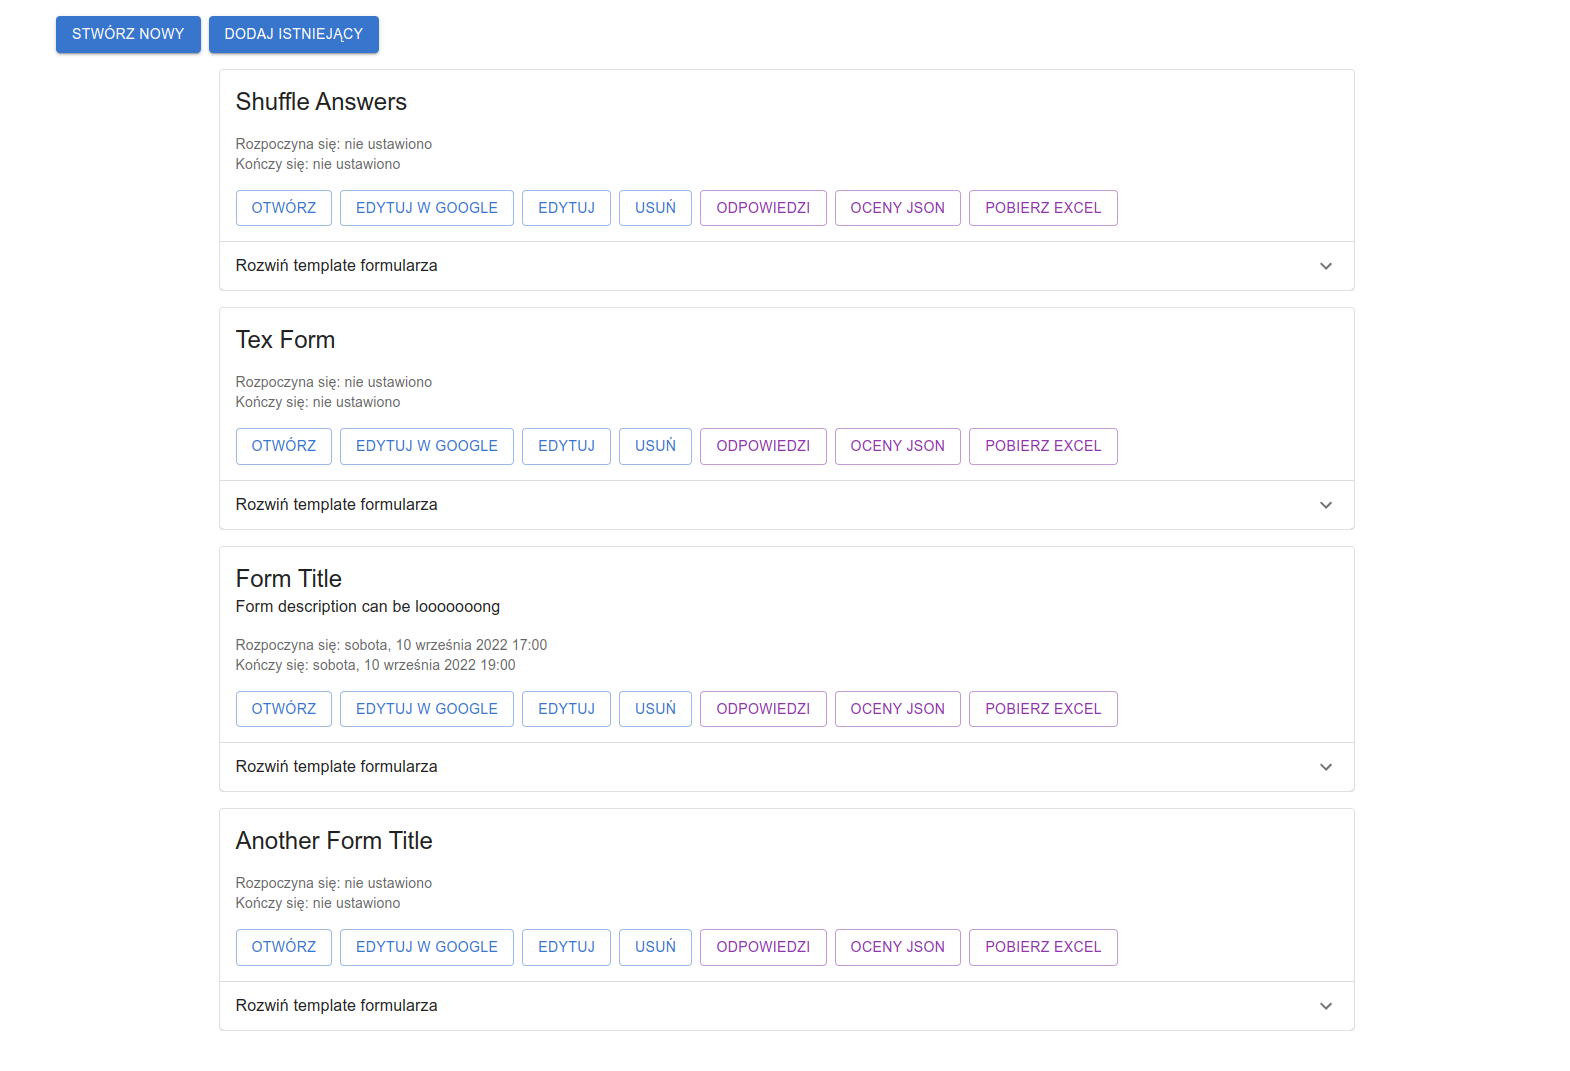
\includegraphics[scale=0.26]{strona.png}
  \caption{Interfejs aplikacji}
  \label{fig:2}
\end{figure}
Przycisk ,,Stwórz nowy'' otworzy dialog, w którym należy wprowadzić kodowanie 
formularza i ewentualnie czas rozpoczęcia i zakończenia testu. Po kliknięciu 
,,Stwórz'' na dysku Google zostanie stworzony nowy formularz i wpis o nim pojawi
się na liście na głównej stronie aplikacji. Przycisk ,,Dodaj istniejący'' otworzy
dialog, gdzie możemy podać identyfikator istniejącego już formularza, który chcemy
dodać do listy formularzy zarządzanych przez aplikację. Musimy również podać jego
kodowanie. Po kliknięciu ,,Dodaj'' formularz zostanie edytowany. 
Na liście formularzy każdy wpis odpowiada jednemu formularzowi
na dysku Google użytkownika, jednak nie wszystkie formularze na dysku się tu pojawią,
jedynie te stworzone przez aplikację lub dodane używając przycisku ,,Dodaj istniejący''.
W każdym wpisie możemy znaleźć przyciski:
\begin{itemize}
  \item ,,Otwórz'': otwiera formularz na stronie Google w nowej karcie,
  \item ,,Edytuj w Google'': otwiera stronę edycji formularza na stronie Google
    w nowej karcie,
  \item ,,Edytuj'': otwiera dialog, gdzie można edytować kodowanie formularza,
  \item ,,Usuń'': usuwa formularz z listy formularzy zarządzanych przez aplikację
    i usuwa całą jego zawartość, jednak pusty formularz tylko z tytułem pozostanie 
    na dysku Google użytkownika,
  \item ,,Odpowiedzi'': pokazuje wszystkie przesłane odpowiedzi, łącznie z tymi
    przesłanymi przed początkiem lub po końcu ustawionych w kodowaniu formularza,
  \item ,,Oceny JSON'': wyświetla ocenione odpowiedzi bez pytań otwartych w formacie
    JSON,
  \item ,,Pobierz Excel'': pobiera plik Excel z ocenionymi zamkniętymi pytaniami,
  \item ,,Rozwiń template formularza'': podgląd kodowania formularza,
\end{itemize}

\subsection{Przeprowadzanie egzaminów}
Jeśli narzędzie ma być użyte do przeprowadzenia egzaminu na początku należy stworzyć
z jego pomocą pusty formularz tylko z tytułem, ewentualnie krótką informacją o czasie
startu. Przed rozpoczęciem należy ręcznie włączyć w ustawieniach formularza na stronie
Google zbieranie adresów email i ewentualnie tasowanie pytań. Następnie w momencie
rozpoczęcia egzaminu należy go zaktualizować dodając do niego pytania.
Po czasie zakończenia egzaminu można go ręcznie zamknąć, ale jeśli ma zostać użyte
automatyczne ocenianie, nie wolno zmieniać jego kodowania w aplikacji. Narzędzie
przefiltruje przesłane odpowiedzi i automatycznie je oceni po kliknięciu
odpowiedniego przycisku.

